\section{Systematic Errors}

In this section we will estimate (or set upper limits on) the contributions to the systematic uncertainty for this experiment.
The sources of systematic uncertainties from the experimental setup (target, acceptance, inelastic contamination) were already estimated for the SBS \gmn experiment proposal~\cite{E12-09-019}.
Note that a majority of the potential sources of systematic uncertainties (nuclear corrections, accidentals, radiative corrections, target density, etc) cancel in the ratio $R = f_{corr} \times N_{e,e'n}/N_{e,e'p}$, which is one of the strengths of this experimental method.
The sources of uncertainties as well as their estimation for each kinematic is provided in Table.~\ref{r_systematic_summary}.
Since the experimental setup has evolved since then, some of these uncertainties have been reevaluated, namely the acceptance loss and inelastic contamination.
%
\begin{table}[!h]
\begin{center}
\caption{
  Estimated contributions (in percent) to the systematic error on $R = f_{corr} \times N_{e,e'n}/N_{e,e'p}$.  
  Quantities marked with $^*$ are taken from the SBS \gmn experiment proposal~\cite{E12-09-019}.
  The total systematic errors on $R$ is the quadratic sum of all other errors.
}
\label{r_systematic_summary}
\vspace{.2in}
{\begin{tabular}{|l|c|c|c|c|}
\hline
\hline
 Kinematic & {\bf 1+} & {\bf 2+} & {\bf 3+}/{\bf 3-} & {\bf 4+}/{\bf 4-}\\
\hline
% Radiative corrections & \multicolumn{2}{|c|}{?} \\
%\hline
% Nuclear correction$^*$ & \multicolumn{2}{|c|}{-} \\
%\hline
%Accidentals$^*$ & \multicolumn{2}{|c|}{-} \\
%\hline
%Target windows$^*$ & \multicolumn{2}{|c|}{0.2 \%} \\
\hline
Acceptance losses & 0.5 \% & 3.0 \% & 0.6 \% & 3.2 \\
\hline
Inelastic contamination & 0.9 \% & 0.6 \% & 1.0 \% & 0.7 \% \\
\hline
Nucleon mis-identification$^*$ & \multicolumn{4}{|c|}{0.6 \% } \\
\hline
%HCal calibration & \multicolumn{2}{|c|}{0.5} \\
%\hline
\hline
%Syst. error on \gmnc/{G$^{\mbox{\scriptsize p}}_{_{\mbox{\tiny M}}}~$}&
Syst. error on $R = f_{corr} \times N_{e,e'n}/N_{e,e'p}$ & 1.2 \%  & 3.1 \% & 1.3 \%  & 3.3 \%  \\
(Quadratic sum of the errors above) & & & &  \\
\hline
\hline
\end{tabular}}
\end{center}
\end{table}
%
%
\begin{table}[!h]
\begin{center}
\caption{
  Estimated contributions to systematic error on the Rosenbluth slope.
}
\label{ntpe_systematic_summary}
\vspace{.2in}
{\begin{tabular}{|l|c|c|}
\hline
\hline
& \qsq~= 4.5 \gevcsq~ & \qsq~= 3.0 \gevcsq~ \\
\hline
Syst. error on $p$ cross section ($S^p = \sigma_{L}^p/ \sigma_{T}^p$) & 0.01 & 0.01 \\
\hline
Syst. error on $n$ form factor ($\mu_n$\gen/\gmn) & 0.05 & 0.041\\
\hline
\hline
Syst. error on Rosenbluth slope (TPE) & 0.012 &  0.011 \\
\hline
\hline
\end{tabular}}
\end{center}
\end{table}
%
Table.~IV %~\ref{ntpe_systematic_summary}
lists the estimated contributions to systematic errors on the two-photon-exchange contribution (TPE).
The systematics for $S^p$ and $\mu_n$\gen/\gmn have already been explicited in Sec.~\ref{sec:exp_method}, and are the leading contributions to the total uncertainty.

%Inelastic contamination has been reevaluated in Sec.~\ref{sec:inel_contam}.
To evaluate the upper limit on our uncertainty, we added quadratically the inelastic contamination evaluated for the proton and the neutron for each kinematics. This would be the error that we make on $R$ if we ignore the inelastic contamination in the quasi-elastic $e-n$ and $e-p$ samples. Even in this case, we expect less than 1\% systematic errors. Of course, we do plan to reevaluate and subtract the inelastic contamination from our actual data sample, so the quoted systematic uncertainty coming from inelastic contamination should be a upper limit.
In the analysis of NTPE/E12-20-010, the inelastic contamination is subtracted from our samples by different methods, which provide very similar results. In practice, the systematic from inelastic, while being carefully evaluated, is within the ball park of the percent;

The acceptance loss in SBS ({\it i.e.} the proportion of non-detected nucleons for each detected electron) have been evaluated for both kinematics.
They are about 10\% for the $\epsilon = 0.60$ kinematic (meaning that for every good electron measured, we will not measure the recoil nucleon 10\% of the times), but they are over 30 \% for the $\epsilon= 0.84$ kinematics, which is due to a larger spread of the nucleon imprint.
The systematic uncertainty on the acceptance loss for the ratio $R = f_{corr} \times N_{e,e'n}/N_{e,e'p}$ is maximized by the proton-neutron solid angle asymmetry $A_{\Delta\Omega} = {\Delta\Omega_n-\Delta\Omega_p}/{\Delta\Omega_n+\Delta\Omega_p}$.
This asymmetry is about~0.5\% for the $\epsilon = 0.60$ kinematic (consistent with the \gmn proposal), but goes up to~3\% for the $\epsilon= 0.84$ kinematics.
In practice, in the analysis of NTPE/E12-20-010 this acceptance loss is being alleviated entirely by the application of a fiducial cut that rejects all events where either the proton or the neutron are out of the acceptance (see Fig.~14.)%\ref{fig:fidcut}). 
%
\begin{figure}[!h]
  \centering
    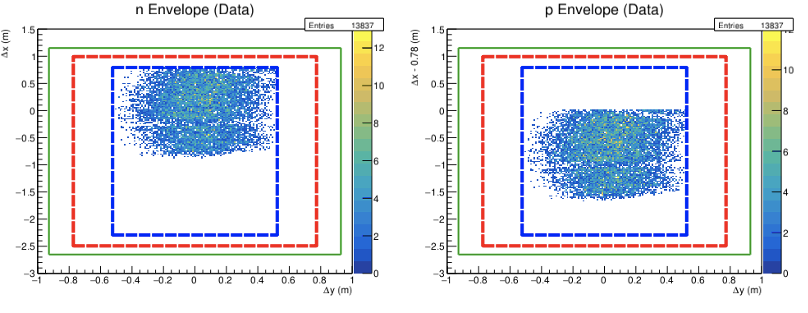
\includegraphics[width=12cm]{Plots/FiducialCut.png}
    \caption{Fiducial cut applied on the NTPE data: These are the distributions of events projected nucleon position in the HCAL surface. The green limit is the HCal boundary, the red limit is the ``active'' region, and the blue limit is the fiducial cut, that ensures that we keep the events where both the projected proton and projected neutron are inside the active region.}
    \label{fig:fidcut}
\end{figure}
%
%\subsection{Acceptance Losses}



